\documentclass{protokoll}
\usepackage{booktabs,multirow,xspace,gnuplot-lua-tikz}
\newcommand{\assistent}{M. Schmitz}
\newcommand{\versuch}{ATLAS}
\newcommand{\nummer}{E214}

\lstset{language=[Visual]C++,
basicstyle=\footnotesize,       % the size of the fonts that are used for the code
backgroundcolor=\color{white},  % choose the background color. You must add \usepackage{color}
tabsize=2,	                % sets default tabsize to 2 spaces
captionpos=b,                   % sets the caption-position to bottom
breaklines=true,                % sets automatic line breaking
breakatwhitespace=false,        % sets if automatic breaks should only happen at whitespace
escapeinside={\%*}{*)},          % if you want to add a comment within your code
keywordstyle=\color{blue}\bfseries,
commentstyle=\color{MidnightBlue}\itshape,
basicstyle=\footnotesize
}

\begin{document}

\section{Einleitung}
In diesem Praktikumsversuch soll die Physik des ATLAS-Experimentes kennengelernt und untersucht werden. So wird sich einleitend anhand von \emph{event displays} mit den zu Grunde liegenden Prozessen und dem ATLAS vertraut gemacht. Anschlie�end wird die Messung der Elektronenenergie anhand der $Z^0$-Masse kalibriert, woraufhin dann entweder eine Bestimmung der W-Boson-Masse oder aber die Suche nach neuer Physik anhand von simulierten ATLAS Daten erfolgt.

\section{Theoretische Grundlagen}
\subsection{Das Standardmodell}
\subsubsection{Teilchen}
\subsubsection{Wechselwirkungen}

\subsection{Neue Physik}

\subsection{Kinematik}

\subsection{Der LHC}

\subsection{ATLAS}

\subsection{Koordinatensysteme}
Bei der Wahl eines angemessenen Koordinatensystems bieten sich im Wesentlichen drei an. Zum einen besteht die M�glichkeit in einem kartesischen Koordinatensystem die Strahlrichtung als z-Achse zu w�hlen, zum Mittelpunkt des LHC-Ringes zeigt die x-Achse und orthogonal auf beiden steht die y-Achse.
Zum anderen steht die Wahl eines kanonischen Kugelkoordinatensystems zur Verf�gung. Da jedoch die Ereignisse nicht gleichverteilt auftreten, sondern auf Grund der nur geringen Transversalimpulse eine H�ufung bei kleinen Winkeln zu erwarten ist, modifiziert man das Koordinatensystem und f�hrt eine neue Gr��e ein, die Rapidit�t $y \equiv \frac{1}{2} \ln{\frac{E+p_z}{E-p_z}}$. Rapidit�tsdifferenzen sind invariant unter Lorentz-Boosts parallel zu z-Achse. In Systemen in denen die Partonenmassen vernachl�ssigt werden k�nnen erh�lt man mit dem Winkel $\theta$ zur Strahlachse stattdessen die sogenannte Pseudo-Rapidit�t
\begin{align}
\eta = - \ln{\left(\tan{\frac{\theta}{2}}\right)}  \ \ldotp
\end{align}
Der ATLAS-Detektor kann Pseudo-Rapidit�ten $|\eta| < 2.5$ f�r Leptonen sowie $|\eta| < 5$ f�r Hadronen aufl�sen.


\section{Aufgaben vor Versuchsbeginn}
\subsection*{Frage A: Zerfall des $Z^0$-Bosons}
\emph{Welchen Wert hat der Impuls eines Elektrons beim Zerfall des $Z^0$-Bosons ($Z^0 \rightarrow e^+ e^-$) im Ruhesystem des $Z^0$-Bosons?}

Das $Z^0$-Boson wird in Ruhe betrachten, hat also einen verschwindenden Dreier-Impuls $\vec{p}_Z$. Da Vierer-Impuls-Erhaltung gilt, verschwindet auch die Summe der Dreier-Impulse von Positron und Elektron ($\vec{p}_{e^+} = - \vec{p}_{e^-}$). Man betrachte also die 0-Komponente der Vierer-Impulse:

%noch sch�ner machen:
\begin{eqnarray*}
               E_{Z^0} &=& E_{e^+} + E_{e^-} \\
\Rightarrow  m^2_{Z^0} &=& 2 E_{e^-} \\
                       &=& 2 \sqrt{m^2_e + \vec{p_e}^2} \\
\Rightarrow  \vec{p_e}^2 &=& \frac{m^2_{Z^0}}{4} - m^2_e \\
\Rightarrow  \vec{p_e}   &=& \sqrt{\frac{m^2_{Z^0}}{4} - m^2_e} \\
                         &=& \unit[45.6]{GeV}
\end{eqnarray*}

\subsection*{Frage B: Elektron-Positron-Streuung}
\emph{Wie gro� ist der Impuls der $\tau$-Leptonen bei der Reaktion $e^+ e^- \rightarrow \tau^+ \tau^-$ im CMS ($\sqrt{s} = \unit[5]{GeV}$)?}

Es gilt Energieerhaltung ($s = s'$), somit folgt:
\begin{eqnarray*}
    \sqrt{s} &=& E_{\tau^+} + E_{\tau^-} \\
             &=& 2 E_{\tau^+} \\
             &=& 2 \sqrt{m^2_{\tau} + p^2_{\tau}} \\
\Rightarrow  p^2_{\tau} &=& \frac{s}{4} - m^2_{\tau} \\
\Rightarrow  p_{\tau}   &=& \sqrt{\frac{s}{4} - m^2_{\tau}} \\
\Rightarrow  p_{\tau}   &=& \unit[1.76]{GeV}
\end{eqnarray*}

\subsection*{Fragen zu Versuchsteil 2}
\emph{Wie kann der Transversalimpuls des W-Bosons bestimmt werden? Wie k�nnen Sie die Variable} \texttt{ptw} \emph{aus den anderen ROOT-Variablen bestimmen?}
%antwort

\emph{Leiten Sie aus Gleichung (4.4) die Gleichung (4.5) her.~\cite{skript}}
%antwort

\subsection*{Fragen zu Versuchsteil 3}
%...

\subsection*{Fragen zu Versuchsteil 4}
\emph{Was ist die minimale invariante Masse der vier Leptonen aus einem $Z^0$-Paar? Weshalb findet man auch unterhalb dieser Schwelle Vier-Lepton-Ereignisse?}
%antwort

\emph{Ein \textsc{Higgs}-Boson zerfalle in zwei $Z^0$. Wie sieht die Verteilung der invarianten Masse der vier Leptonen aus?}
%antwort

\emph{Ein idealer Detektor wird vorrausgesetzt. Welches ist das typische $\slash{E}_T$, wenn ein $Z^0$-Paar in Elektronen oder Myonen-Paare zerf�llt? Wie wird $\slash{E}_T$ bei einem realen Detektor aussehen?}
%antwort

\emph{noch ne frage ...}
%antwort

\emph{un noch eine ...}
%antwort


\section{Versuchsdurchf�hrung und Auswertung}
\subsection{Teil 2: Kalibration der Elektronen}\label{subsec:ElektronKalibration}
Die genauste Methode um die Energie eines Elektrons zu bestimmen, ist die Messung der Energie des elektromagnetischen Schauers, den das Elektron im Kalorimeter ausl�st. Da das Kalorimeter aus vielen hundert Einzelteilen besteht, die alle verschiedene Eigenschaften haben und aufgrund systematischer Energieverluste durch inaktive Regionen im Detektor und Energieverluste der Elektronen bevor sie das Kalorimeter erreichen, muss diese Energiemessung kalibriert werden. Diese Kalibration l�sst sich aufgrund der sehr genau bekannten Eigenschaften des $Z^0$, anhand dessen Zerfall in ein $e^+e^-$-Paar durchf�hren. Dazu stehen uns Daten solcher gemessener Zerf�lle zur Verf�gung, die wir mithilfe des Programms ROOT analysieren.\\
Zuerst plotten wir ein Histogramm der Invarianten Masse des Elektron-Positron-Paars und fitten eine Voigt Funktion an den erhaltenen Graph (siehe Abbildung \ref{fig:Zee_raw}). Die Voigt-Funktion ist das Ergebnis einer Faltung der Breit-Wigner-Resonanzkurve mit einer Gau�verteilung, die die Verbreiterung der Kurve durch Detektoreffekte approximiert. Wie erwartet zeigt der Graph einen Peak, der aufgrund der mangelnden Kalibration der Energiemessung nicht genau mit der $Z^0$ Masse �bereinstimmt. 
\begin{figure}[H]
	\centering
		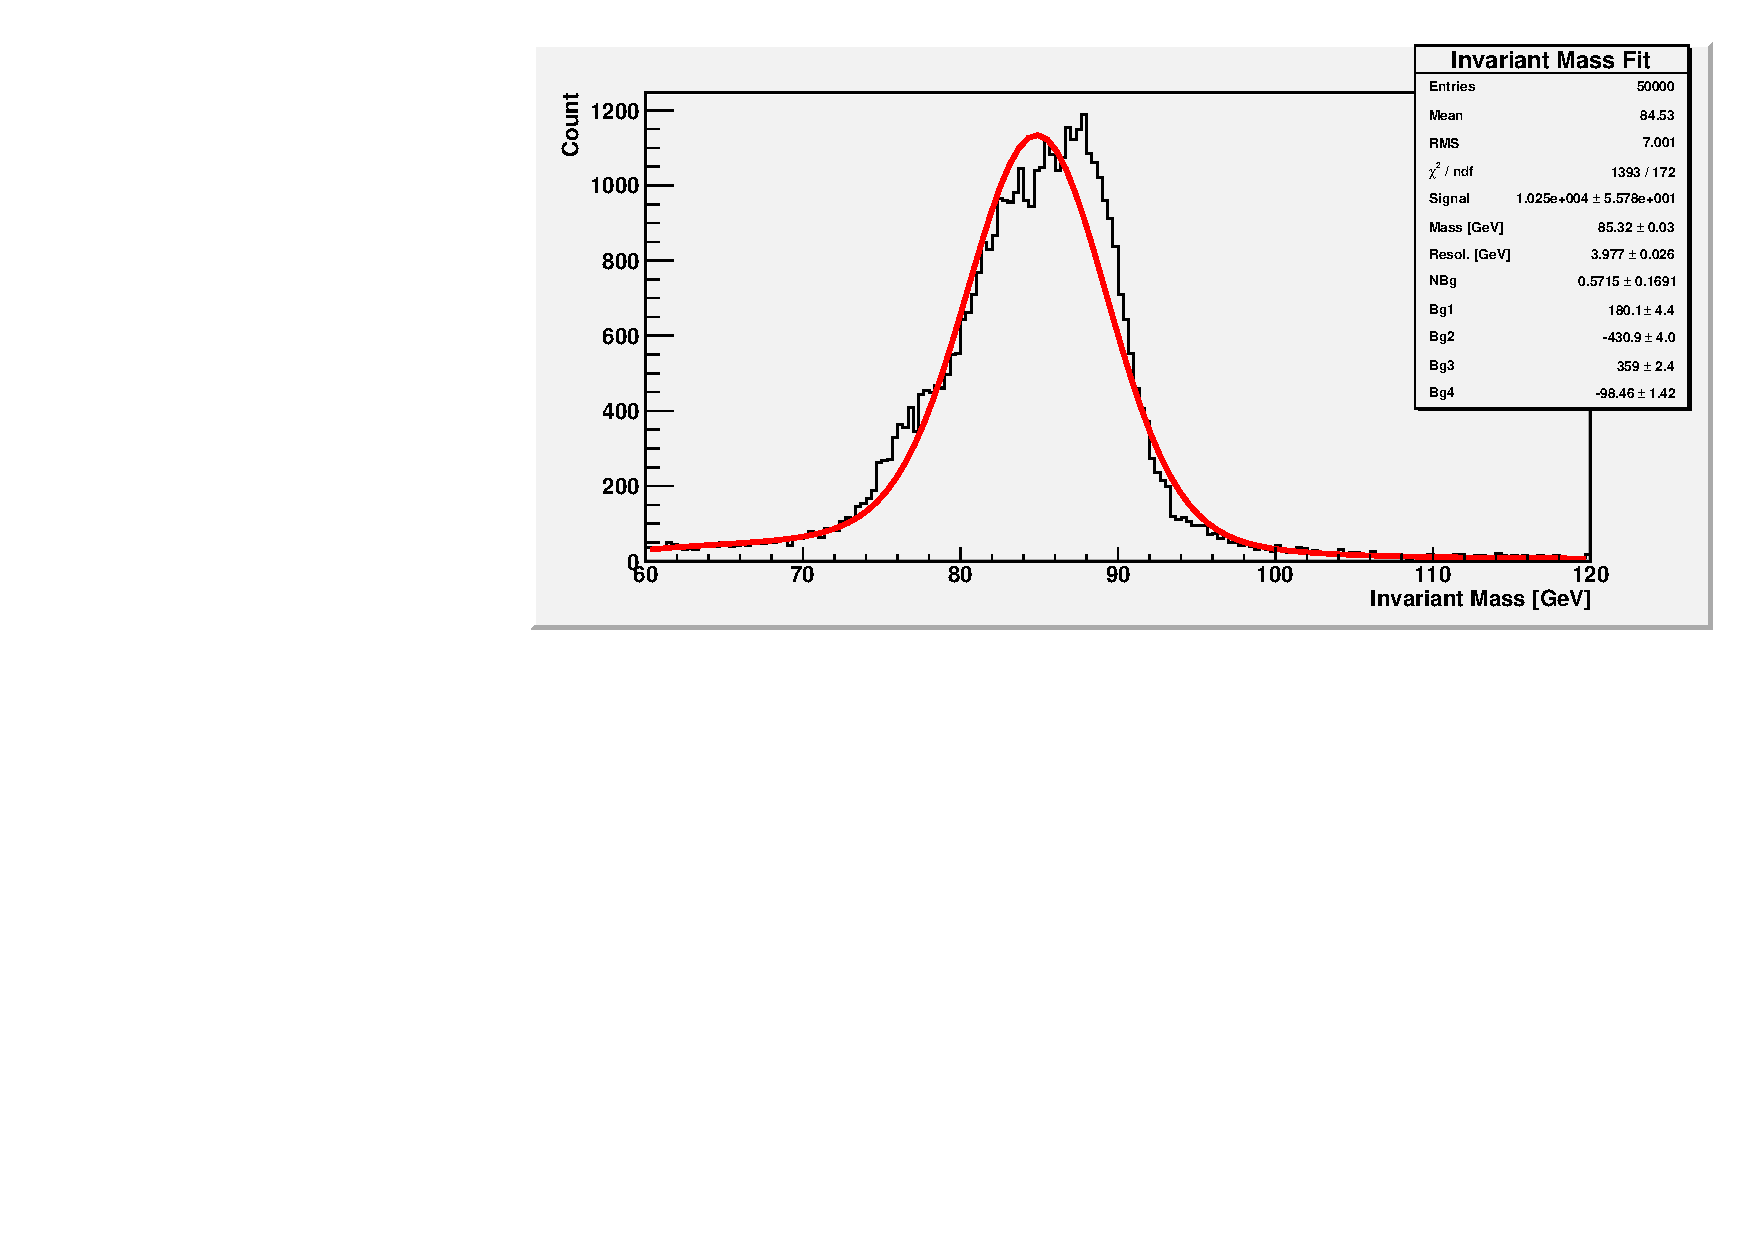
\includegraphics[width=0.8\textwidth]{Zee_raw.pdf}
	\caption{Invariante Masse des Leptonpaars beim Zerfall $Z^0\rightarrow e^+e^-$ mit unkalibrierter Energiemessung.}
	\label{fig:Zee_raw}
\end{figure}
Zur Kalibration betrachtet man nun die Position des $Z^0$ Peaks in Abh�ngigkeit verschiedener Variablen, anschlie�end kann man diese durch Multiplikation der Energiewerte mithilfe eines C++ Scriptes auf die bekannte $Z^0$ Masse korrigieren. Im C++ Script stehen folgende Variablen zur Verf�gung:
\begin{itemize}
\item $E_\textit{raw}$: Die unkalibrierte Energie.\\
\item $pt$: Der transversale Impuls.\\
\item $phi, eta$: Richtung des Elektrons (azimutaler Winkel $\phi$ und $\eta$).\\
\item $etiso$: Transversale Energie im Kalorimeter in der Umgebung des Elektrons.\\
\item $eoverp$: Verh�ltnis zwischen Elektron-Energie und -Impuls.\\
\item $drjet$: Abstand des Elektrons zum n�chsten Jet (in der $\eta\phi$ Ebene)
\end{itemize}
Als Beispiel sei in Abbildung \ref{fig:Zee_eta} die gemessene $Z^0$ Resonanz f�r verschiedene $\eta$-Bereiche dargestellt.
\begin{figure}[H]
	\centering
		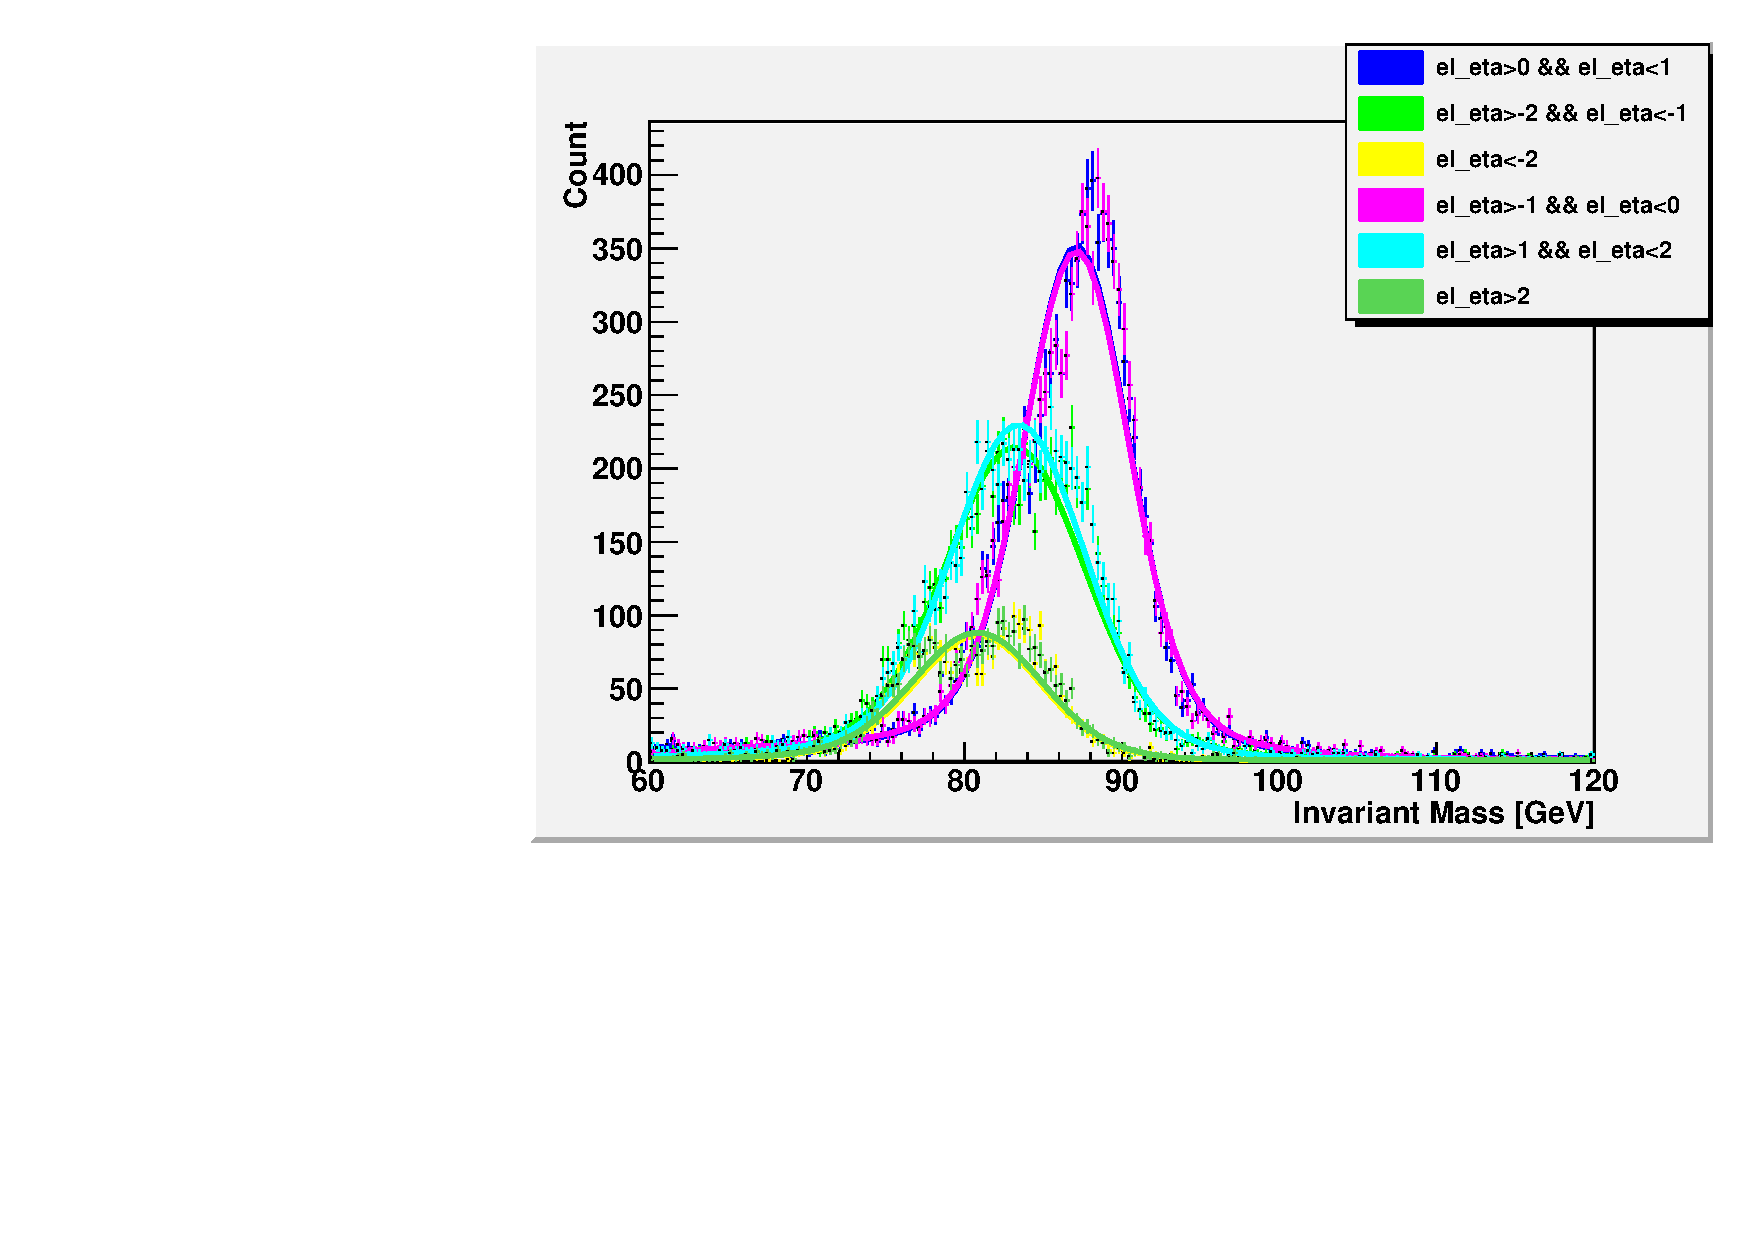
\includegraphics[width=0.8\textwidth]{Zee_eta.pdf}
	\caption{Invariante Masse des Leptonpaars beim Zerfall $Z^0\rightarrow e^+e^-$ f�r verschiedene Bereiche der Pseudorapidit�t $\eta$ des Elektrons vor der Kalibration.}
	\label{fig:Zee_eta}
\end{figure}
F�r die verschiedenen $\eta$ Bereiche lassen sich nun verschiedene Multiplikatoren f�r die Energiewerte bestimmen um die $Z^0$ Resonanz jeweils auf den richtigen Wert zu verschieben. Dieses Verfahren kann man iterativ auch auf die anderen Variablen anwenden. Das von uns auf diese Weise geschriebene Skript findet sich im Anhang \ref{subsec:eleccalib}. In Abbildung  \ref{fig:Zee_eta_calib} ist analog zu Abbilung \ref{fig:Zee_eta} die gemessene $Z^0$ Resonanz f�r verschiedene Werte von $\eta$ nach der Kalibration dargestellt. In Abbilung \ref{fig:Zee_calib} findet sich der Fit an die Gesamtverteilung nach der Kalibration mit den Fitparametern. Die gemessene $Z^0$ liegt nun mit $91.17 \pm 0.02$ GeV sehr gut vertr�glich mit dem Literaturwert von $91.1876 \pm 0.0021$ GeV. Die Aufl�sung des Detektors hat sich von $3.977 \pm 0.026$ GeV auf $1.963 \pm 0.02$ GeV verbessert. 
\begin{figure}[H]
	\centering
		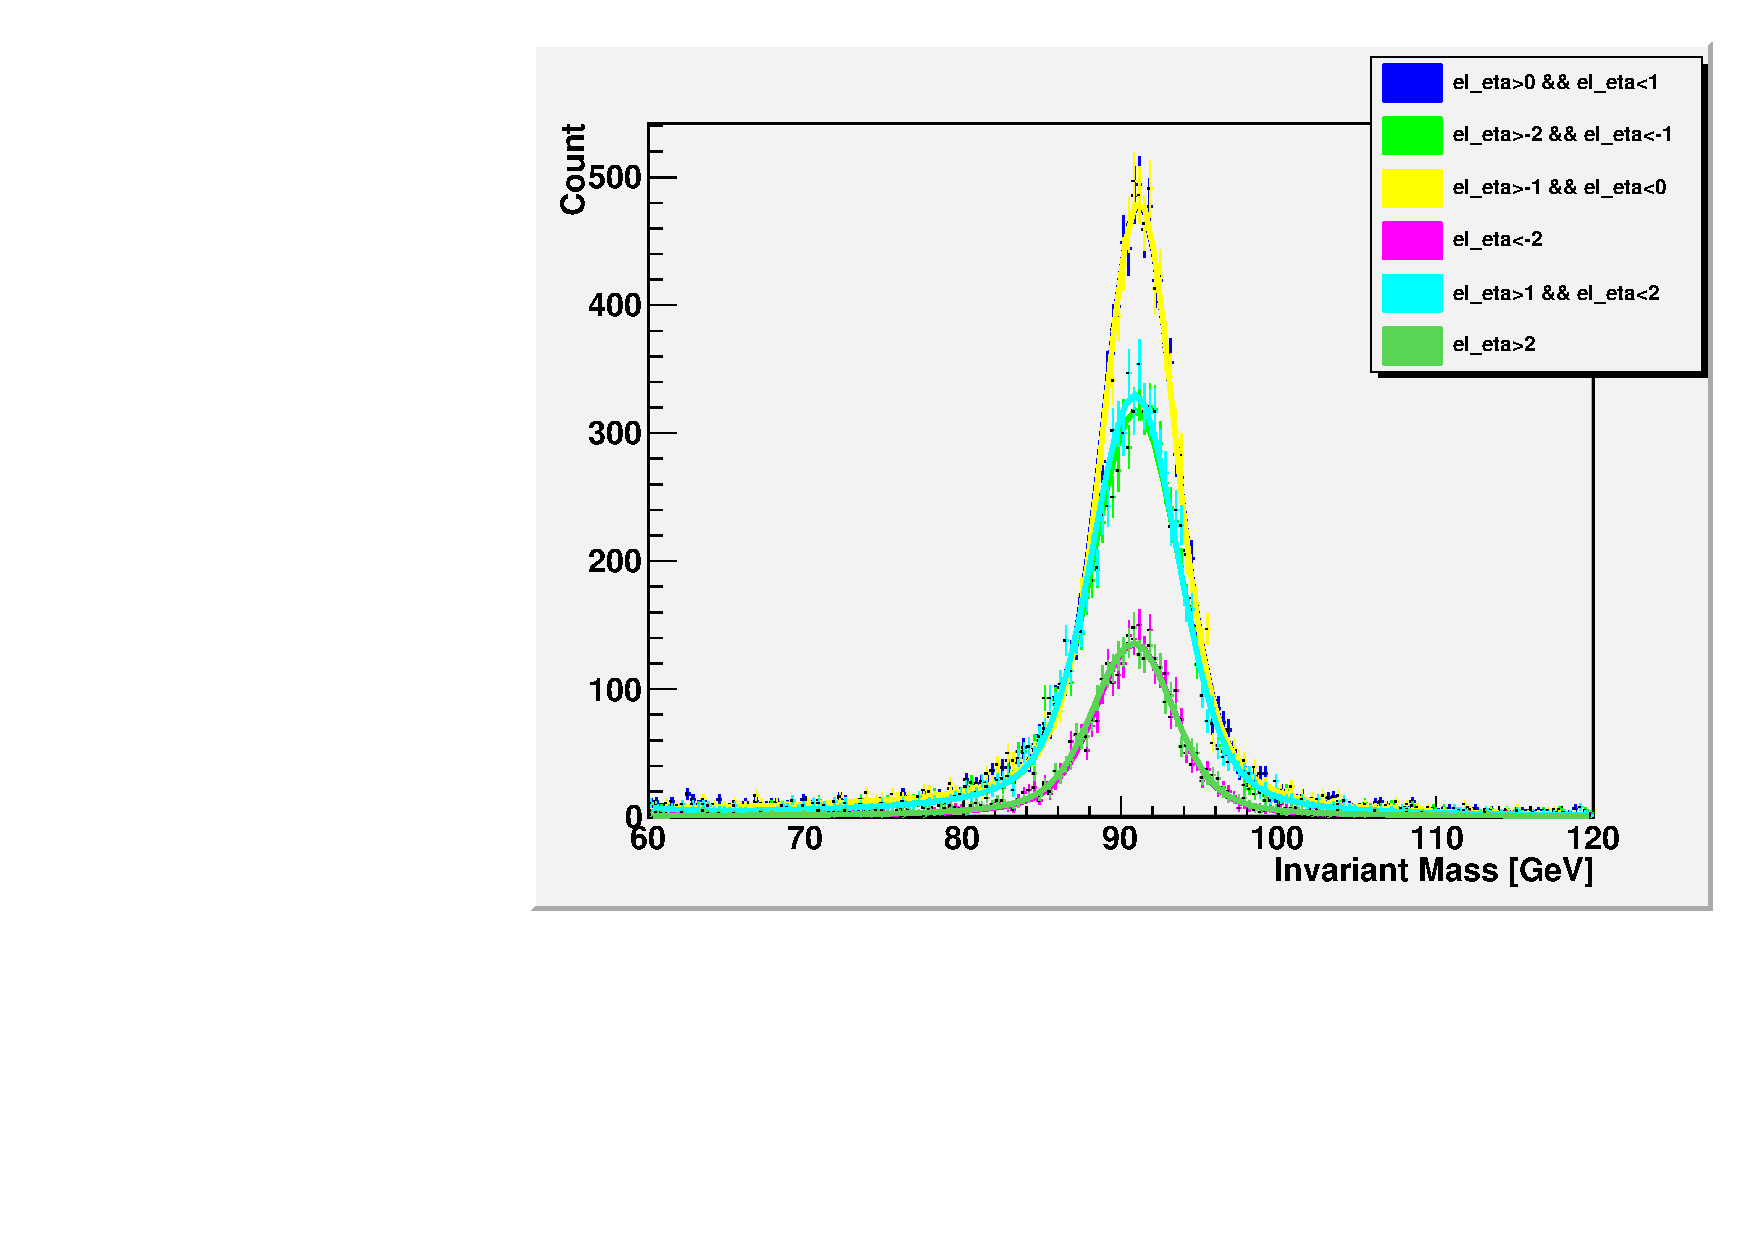
\includegraphics[width=0.8\textwidth]{Zee_eta_calib.pdf}
	\caption{Invariante Masse des Leptonpaars beim Zerfall $Z^0\rightarrow e^+e^-$ f�r verschiedene Bereiche der Pseudorapidit�t $\eta$ des Elektrons nach der Kalibration.}
	\label{fig:Zee_eta_calib}
\end{figure}
\begin{figure}[H]
	\centering
		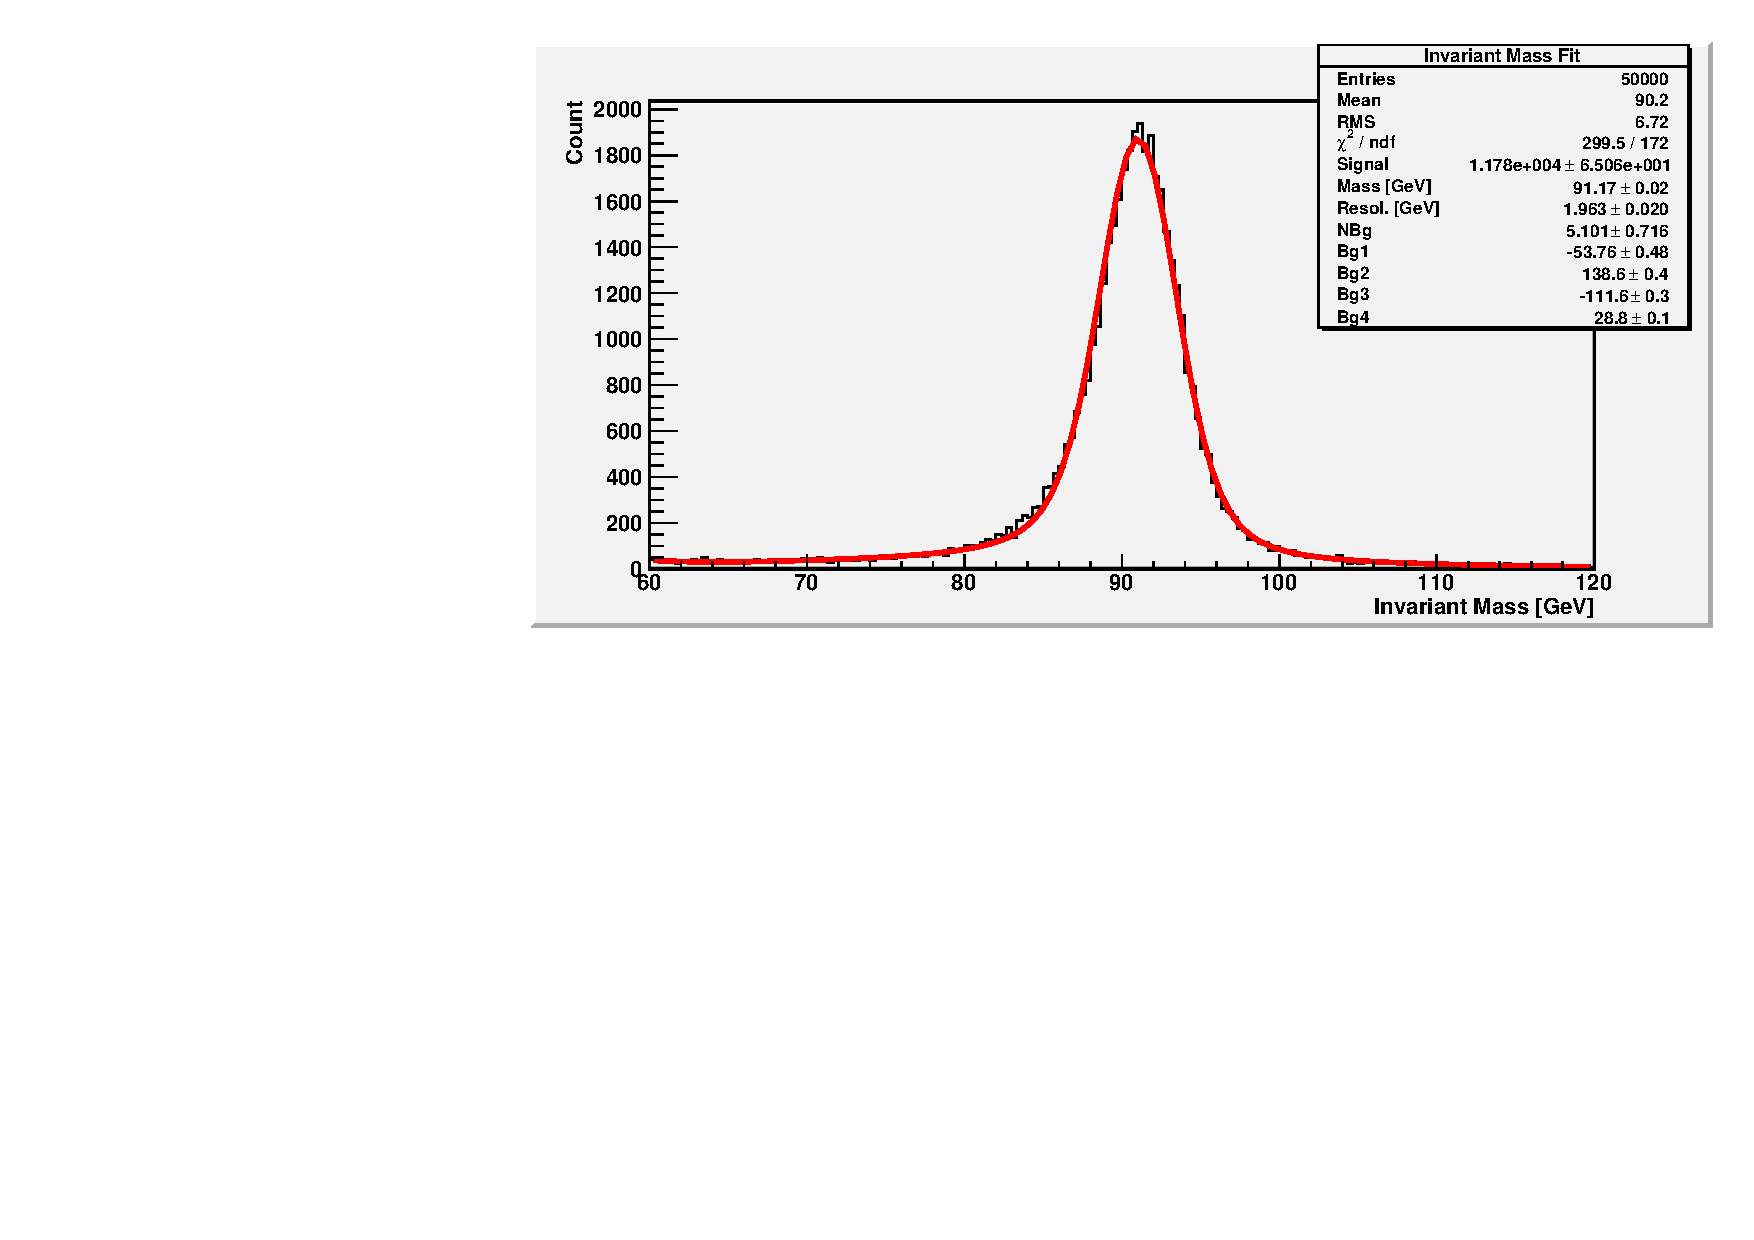
\includegraphics[width=1.0\textwidth]{Zee_calib.pdf}
	\caption{Invariante Masse des Leptonpaars beim Zerfall $Z^0\rightarrow e^+e^-$ nach der Kalibration mit VoigtFit und Parametern.}
	\label{fig:Zee_calib}
\end{figure}
\section{Zusammenfassung}

\begin{appendix}
  \section{Quellcode}\label{sec:sourcecode}
\subsection{ElecCalib.cpp}\label{subsec:eleccalib}
\begin{lstlisting}
double ElecCalib(double e_raw, double pt, double eta, 
		 double phi, double etiso, double eoverp, double mindrjet)
{
  double energy = e_raw;
  if ((eta)>2.0) energy = energy * 91.1876/81.25*91.1876/88.93*91.1876/90.41*91.1876/90.87;
  else if ((eta)>1.5) energy = energy * 91.1876/82.03*91.1876/89.06*91.1876/90.3*91.1876/90.77;
  else if ((eta)>1.0) energy = energy * 91.1876/85.25*91.1876/90.88*91.1876/91.28*91.1876/91.29;
  else if ((eta)>0.0) energy = energy * 91.1876/88.29*91.1876/91.67*91.1876/91.42*91.1876/91.27;
  else if ((eta)>-1.0) energy = energy * 91.1876/91.2641*91.1876/88.4924*91.1876/91.2573*91.1876/91.4781*91.1876/91.3602;
  else if ((eta)>-1.5) energy = energy * 91.1876/91.1872*91.1876/85.7911*91.1876/90.4713*91.1876/91.1639*91.1876/91.2424;
  else if ((eta)>-2.0) energy = energy * 91.1876/90.7617*91.1876/82.0698*91.1876/88.7481*91.1876/90.4027*91.1876/90.869;
  else if ((eta)>-2.5) energy = energy * 91.1876/90.8539*91.1876/81.5198*91.1876/88.6939*91.1876/90.4605*91.1876/90.8548;

  if (fabs(phi)>2.0) energy = energy * 91.1876/91.3577*91.1876/91.1852;
  else if (fabs(phi)>1.5) energy = energy * 91.1876/91.2691*91.1876/91.1819;
  else if (fabs(phi)>1.0) energy = energy * 91.1876/91.2028*91.1876/91.253;
  else if (fabs(phi)>0.0) energy = energy * 91.1876/91.2374*91.1876/91.2807;

  if (pt>75) energy = energy * 91.1876/90.3534*91.1876/90.8199*91.1876/90.9337*91.1876/91.0716;
  else if (pt>50) energy = energy * 91.1876/91.2934*91.1876/91.2528*91.1876/91.2152*91.1876/91.1986;
  else if (pt>25) energy = energy * 91.1876/91.1039*91.1876/91.1697*91.1876/91.1801*91.1876/91.1844;
  else if (pt>0) energy = energy * 91.1876/91.4275*91.1876/91.2845*91.1876/91.2393*91.1876/91.2064;

  if (eoverp>7.5) energy = energy*91.1876/92.5439*91.1876/92.3647*91.1876/92.5107;
  else if (eoverp>5.0) energy = energy*91.1876/91.3806*91.1876/91.3122*91.1876/91.3581;
  else if (eoverp>2.5) energy = energy*91.1876/90.3963*91.1876/90.334*91.1876/90.3737;
  else if (eoverp>0) energy = energy*91.1876/91.1876*91.1876/91.1876*91.1876/91.1876;

  if (etiso>1.5) energy = energy*91.1876/91.3671*91.1876/91.1977;
  else if (etiso>1.0) energy = energy*91.1876/91.3977*91.1876/91.2983;
  else if (etiso>0.5) energy = energy*91.1876/91.3588*91.1876/91.2324;
  else if (etiso>0) energy = energy*91.1876/91.1515*91.1876/91.0749;

  if (mindrjet>7.5) energy = energy*91.1876/91.1876*91.1876/91.1876*91.1876/91.1876;
  else if (mindrjet>5.0) energy = energy*91.1876/90.7937*91.1876/91.1729;
  else if (mindrjet>2.5) energy = energy*91.1876/91.1319*91.1876/91.1002;
  else if (mindrjet>0) energy = energy*91.1876/91.0853*91.1876/91.0663;

  return energy;
} 
\end{lstlisting}
  \section{Tabellen}

  \Literatur{quellen}

\end{appendix}
\end{document}
